\section{Input and Output}
The PCB contains a microcontroller used to manage all input and output between the FPGA and the IO devies shown in figure ~\ref{figure:system-overview}.
The microcontroller listens on all IO channels for input, and acts on the input, either forwarding the request to another device or performing memory operations on the FPGA's memory.

\subsection{Communication channels}
\subsubsection{SD Card}
The SD card reader is primarily used as a storage for programs that are to be uploaded on the FPGA.
However, it might also be used to store memory snapshots in order to look how the genetic algorithm converges to a solution over time.
\todo{Reference application note with example code for SD}

The Energy Micro Application Note on Fat and SD cards \todo{cite the application note}, and its example code, describes an implementation of the FatFS library on the Giant Gecko microcontroller.

\paragraph{FatFS}\cite{fatfs-web}

FatFS is a generic FAT file system for microcontrollers, with a generic interface for the FAT operations, and a hardware specific interface for disk I/O.
Because of this structure, the system is easily portable.
To add read and write a FAT system on some disk drive, FatFS needs the following functions:

\begin{table}
    \begin{tabular}{| l | l |}
        \hline
        disk\_initialize & Initialize disk drive \\
        \hline
        disk\_status & Get disk status \\
        \hline
        disk\_read & Read sectors on disk \\
        \hline
        disk\_write & Write sectors on disk \\
        \hline
        disk\_ioctl & Control device dependent features \\
        \hline
        get\_fattime & Get current time for FAT \\
        \hline
    \end{tabular}
    \caption{Overview of disk I/O functions}
\end{table}

\subsubsection{USB}
The USB is the main communication line with a host computer, allowing the host computer to start running programs on the FPGA and recieve snapshots of the memory periodically.
The microcontroller has a built in USB controller~\cite{efm32gg990-datasheet} and energy micro has supplied an application note~\cite{an0065} with code for utilizing the included USB controller in order to act as a USB device.

\subsubsection{Serial}
The serial port is meant as a backup solution in case USB doesn't work, with the exact same opportunities, but with an older, simpler interface.
The micro controller used in the project has a built in UART Receiver/Transmitter\cite{efm32gg990-datasheet} which is easily activated with code from AN0045~\cite{an0045}.

\subsubsection{LEDs and buttons}
The most primitive form of IO we have are the onboard LEDs and buttons.
They allow a quick and easy way to verify that a program is running, and possibly letting the user change execution modes or the program on the FPGA with the buttons.
All code interfacing with the LEDs and buttons are simple code either setting or reading the value of GPIO pins.
The leds are driven by General Purpose IO pins on the SCU, requiring a minimal amount of code in order to get a working output, which is especially handy in the early stages of implementation.

\subsubsection{FPGA}
There are 41 lines between the FPGA and the SCU in order to facilitate communication.
The FPGA has no way of signalling that it wants to output something, so the SCU is responsible for periodically halting the CPU and reading from it's memory.

\subsubsection{J-link}
In order to program and debug the programs on the SCU, we utilise the built-in pins for debugging using J-Link.
\todo{What more to write about this?}
It can also be used as a form of emergency output as it makes it possible to display text that is printed by the program running on the SCU.

\section{FPGA Control}
The only way of communication with the FPGA is with direct memory access to the FPGA's data and instruction memory.
All the data is transfered directly over the SCU's GPIO pins, without any form for memory mapping or built-in bus interfaces.
Since the instruction memory stores 32 bits per address, \todo{Cite fpga chapter on instruction memory}, there are two states for accessing instruction memory, either the upper or the lower half.
The SRAM datasheet~\cite{sram-datasheet} specifies that the data signal has to be stable for at least 10ns in order to complete a write.
This means that it is not necessary to worry about timing when accessing the SRAM since changing the signal more than every 10ns requires a clock speed of 100MHz.

\begin{table}
    \begin{tabular}{| l | l | l |}
        \hline
        Signal & Bus width & \\
        \hline
        FPGA enable & 1 & Enables the FPGA on high, disables it on low\\
        \hline
        FPGA State & 2 & \pbox{20cm}{00: Processor enable\\01: Instruction memory upper half access\\10: Instruction memory lower half access\\11: Data memory access}\\
        \hline
        Chip enable & 1 & The chip enable signal in to the selected memory block.\\
        \hline
        Write enable & 1 & The write enable signal in to the selected memory block.\\
        \hline
        Address & 19 & The adress bus to the selected memory block.\\
        \hline
        Data & 16 & The data bus to the selected memory block.\\
        \hline
        LBUB & 1 & The LB and the UB signal to the selected memory block.\\
        \hline
    \end{tabular}
    \caption{Lines between the SCU and FPGA}
\end{table}

\section{IO Program}
\begin{figure}[H]
    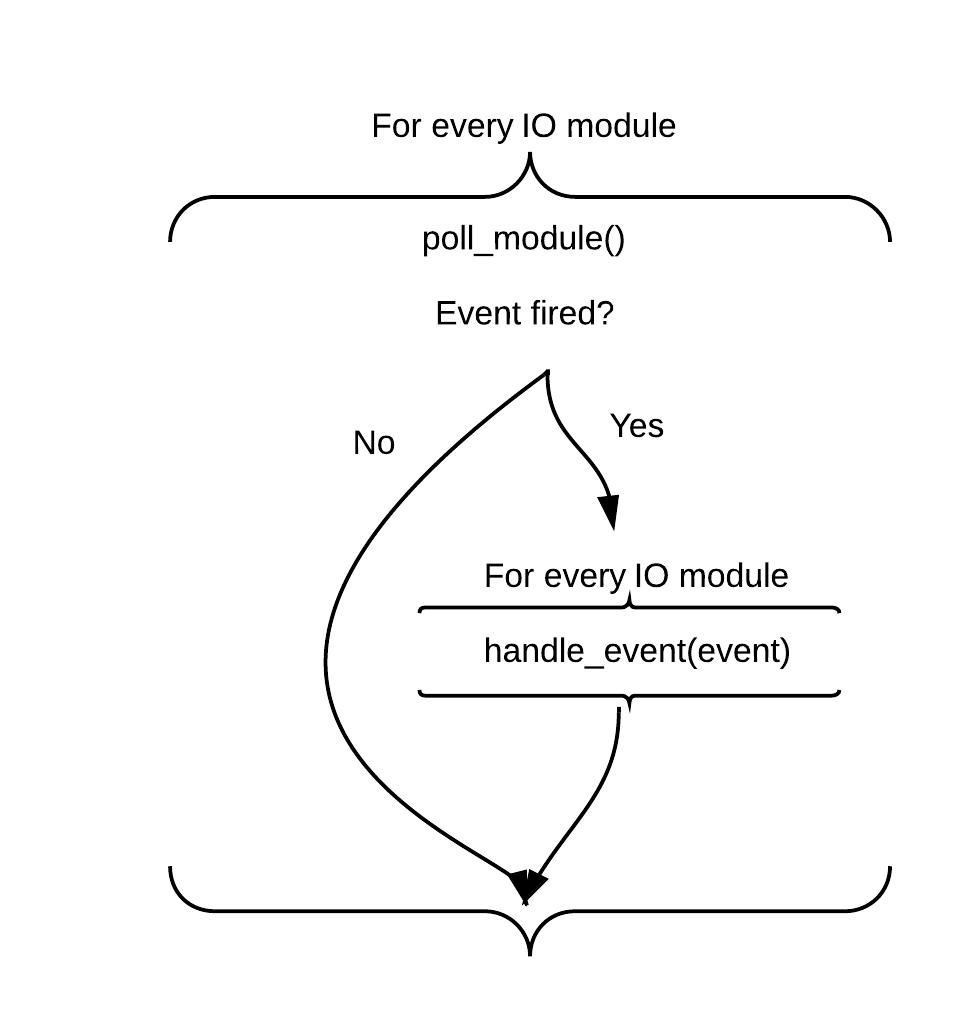
\includegraphics[width=\textwidth]{io/fig/program.png}
    \caption{The body of the IO program's main loop}
\end{figure}

The IO program was designed to be as simple as possible in order to decrease the amount of things that could go wrong.
The main idea is that every IO device is required to define two function, a function that can be called to check whether some input has happened, and a function that is called whenever a device reports input.
In order to enable sending messages between different IO units, the poll functions return a pointer which may point to any object in memory, which allows other modules to read the data given that they know what type of data the pointer points to.

\section{Design decision}
\begin{itemize}
    \item The microcontroller chosen is the same as in the available development kit. As there was no restrictions on power usage, 
          it was decided to use the micro controller most convenient to develop on.
    \item Early in the process, a discussion arised about how it could be beneficial to run an operating system on the micro controller
          such that familiar programs could be used on it. A scenario pitched was to have network access, and then be able to talk to the
          machine remotely using programs such as \textit{SSH} or \textit{telnet}. However, as the Linux version available on the Energy Micro
          system was deemed not so useful, and the controller misses network support, it was decided that running an OS was unnecessarily much work.
    \item FPGA Bus, huge
\end{itemize}

\section{Issues?}
\subsection{Not getting work done}

\subsection{Crystal}

\subsection{USB VBus}

\subsection{No UART}

